A continuación mostramos los modelos $\mu$Modelica equivalentes a los modelos PowerDEVS (junto al icono que lo representa), utilizados para realizar la comparación de performance:

\begin{listing}[H]    
\marginnote{
\includegraphics[width=\marginparwidth]{img/constant_sci}}
     \caption{data/sources/constant\_sci.mo}\label{list:constant_sci.mo}
     \inputminted{modelica}{../../data/sources/constant_sci.mo}
\end{listing} 

\begin{listing}[H]    
\marginnote{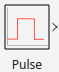
\includegraphics[width=\marginparwidth]{img/pulse_sci}}
	\caption{data/sources/pulse\_sci.mo} \label{list:pulse_sci.mo}
	\inputminted{modelica}{../../data/sources/pulse_sci.mo}
\end{listing} 

\begin{listing}[H]    
\marginnote{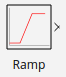
\includegraphics[width=\marginparwidth]{img/ramp_sci}}
	\caption{data/sources/ramp\_sci.mo} \label{list:ramp_sci.mo}
	\inputminted{modelica}{../../data/sources/ramp_sci.mo}
\end{listing} 

\begin{listing}[H]    
\marginnote{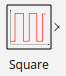
\includegraphics[width=\marginparwidth]{img/square_sci}}
	\caption{data/sources/square\_sci.mo} \label{list:square_sci.mo}
	\inputminted{modelica}{../../data/sources/square_sci.mo}
\end{listing} 

\begin{listing}[H]    
\marginnote{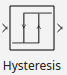
\includegraphics[width=\marginparwidth]{img/hysterectic}}
	\caption{data/qss/hysteretic.mo} \label{list:hysteretic.mo}
	\inputminted{modelica}{../../data/qss/hysteretic.mo}
\end{listing} 

\begin{listing}[H]    
\marginnote{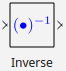
\includegraphics[width=\marginparwidth]{img/inverse_function}}
	\caption{data/qss/inverse\_function.mo} \label{list:inverse_function.mo}
	\inputminted{modelica}{../../data/qss/inverse_function.mo}
\end{listing} 

\begin{listing}[H]    
\marginnote{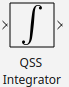
\includegraphics[width=\marginparwidth]{img/qss_integrator}}
	\caption{data/qss/qss\_integrator.mo} \label{list:qss_integrator.mo}
	\inputminted{modelica}{../../data/qss/qss_integrator.mo}
\end{listing} 

\begin{listing}[H]    
\marginnote{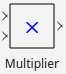
\includegraphics[width=\marginparwidth]{img/qss_multiplier}}
	\caption{data/qss/qss\_multiplier.mo} \label{list:qss_multiplier.mo}
	\inputminted{modelica}{../../data/qss/qss_multiplier.mo}
\end{listing} 

\begin{listing}[H]    
\marginnote{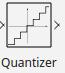
\includegraphics[width=\marginparwidth]{img/qss_quantizer}}
	\caption{data/qss/qss\_quantizer.mo} \label{list:qss_quantizer.mo}
	\inputminted{modelica}{../../data/qss/qss_quantizer.mo}
\end{listing} 

\begin{listing}[H]    
\marginnote{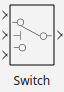
\includegraphics[width=\marginparwidth]{img/qss_switch}}
	\caption{data/qss/qss\_switch.mo} \label{list:qss_switch.mo}
	\inputminted{modelica}{../../data/qss/qss_switch.mo}
\end{listing} 

\begin{listing}[H]    
\marginnote{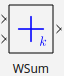
\includegraphics[width=\marginparwidth]{img/qss_wsum}}
	\caption{data/qss/qss\_wsum.mo} \label{list:qss_wsum.mo}
	\inputminted{modelica}{../../data/qss/qss_wsum.mo}
\end{listing} 

\begin{listing}[H]    
\marginnote{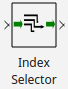
\includegraphics[width=\marginparwidth]{img/IndexSelector}}
	\caption{data/vector/IndexSelector.mo} \label{list:IndexSelector.mo}
	\inputminted{modelica}{../../data/vector/IndexSelector.mo}
\end{listing} 

\begin{listing}[H]    
\marginnote{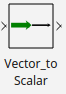
\includegraphics[width=\marginparwidth]{img/vector2scalar}}
	\caption{data/vector/vec2scalar.mo} \label{list:vec2scalar.mo}
	\inputminted{modelica}{../../data/vector/vec2scalar.mo}
\end{listing} 

\begin{listing}[H]    
\marginnote{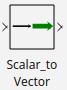
\includegraphics[width=\marginparwidth]{img/scalar2vector}}
	\caption{data/vector/scalar2vec.mo} \label{list:escalar2vec.mo}
	\inputminted{modelica}{../../data/vector/scalar2vec.mo}
\end{listing} 

\begin{listing}[H]    
\marginnote{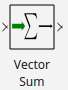
\includegraphics[width=\marginparwidth]{img/vector_sum}}
	\caption{data/vector/vector\_sum.mo} \label{list:vector_sum.mo}
	\inputminted{modelica}{../../data/vector/vector_sum.mo}
\end{listing} 

\begin{listing}[H]    
\marginnote{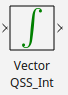
\includegraphics[width=\marginparwidth]{img/qss_integrator_vec}}
	\caption{data/vector/qss\_integrator\_vec.mo} \label{list:qss_integrator_vec.mo}
	\inputminted{modelica}{../../data/vector/qss_integrator_vec.mo}
\end{listing} 

\begin{listing}[H]    
\marginnote{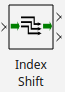
\includegraphics[width=\marginparwidth]{img/index_shift}}
	\caption{data/vector/index\_shift.mo} \label{list:index_shift.mo}
	\inputminted{modelica}{../../data/vector/index_shift.mo}
\end{listing} 

\begin{listing}[H]    
\marginnote{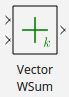
\includegraphics[width=\marginparwidth]{img/qss_sum_vect}}
	\caption{data/vector/qss\_sum\_vec.mo} \label{list:qss_sum_vec.mo}
	\inputminted{modelica}{../../data/vector/qss_sum_vec.mo}
\end{listing} 

\begin{listing}[H]    
\marginnote{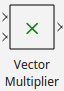
\includegraphics[width=\marginparwidth]{img/qss_multiplier_vec}}
	\caption{data/vector/qss\_multiplier\_vec.mo} \label{list:qss_multiplier_vec.mo}
	\inputminted{modelica}{../../data/vector/qss_multiplier_vec.mo}
\end{listing} 

\begin{listing}[H]    
\marginnote{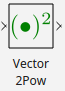
\includegraphics[width=\marginparwidth]{img/vector_pow2}}
	\caption{data/vector/vector\_pow2.mo} \label{list:vector_pow2.mo}
	\inputminted{modelica}{../../data/vector/vector_pow2.mo}
\end{listing} 

\begin{listing}[H]    
\marginnote{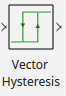
\includegraphics[width=\marginparwidth]{img/hyst_vec}}
	\caption{data/vector/hyst\_vec.mo} \label{list:hyst_vec.mo}
	\inputminted{modelica}{../../data/vector/hyst_vec.mo}
\end{listing} 

\begin{listing}[T]    
\marginnote{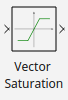
\includegraphics[width=\marginparwidth]{img/vector_sat}}%
	\caption{data/vector/vector\_sat.mo} \label{list:vector_sat.mo}
	\inputminted{modelica}{../../data/vector/vector_sat.mo}
\end{listing} 

